\documentclass[11pt, letterpaper]{article}
\usepackage[utf8]{inputenc}
\usepackage[letterpaper, margin=0.5in]{geometry}
\usepackage{amsmath}
\usepackage{amssymb}
\usepackage{amsthm}
\usepackage{graphicx}
\usepackage{listings}
\usepackage[font=scriptsize]{caption}
\usepackage{subcaption}
\usepackage{xcolor}

\newtheorem{lemma}{Lemma}
\newcommand{\indep}{\perp \!\!\! \perp}

\definecolor{codegreen}{rgb}{0,0.6,0}
\definecolor{codegray}{rgb}{0.5,0.5,0.5}
\definecolor{codepurple}{rgb}{0.58,0,0.82}
\definecolor{backcolour}{rgb}{0.95,0.95,0.92}

\lstdefinestyle{mystyle}{
    backgroundcolor=\color{backcolour},   
    commentstyle=\color{codegreen},
    keywordstyle=\color{magenta},
    numberstyle=\tiny\color{codegray},
    stringstyle=\color{codepurple},
    basicstyle=\ttfamily\footnotesize,
    breakatwhitespace=false,
    texcl=true,
    mathescape=true,
    breaklines=true,                 
    captionpos=b,                    
    keepspaces=true,                 
    numbers=left,                    
    numbersep=5pt,                  
    showspaces=false,                
    showstringspaces=false,
    showtabs=false,                  
    tabsize=2
}

\lstset{style=mystyle}
\graphicspath{ {../statics/} }
\captionsetup{justification=raggedright, singlelinecheck=false}

\author{Ryan Tang}
\title{STA 532 HW 5}
\date{February 20th 2023}

\begin{document}
\maketitle

\section{Chapter 2 Ex 3}
Tropical cyclone study. Here we have the annual counts $X = (X_1 \dots X_n), X_j \thicksim_{iid} \text{Poisson}(\alpha\beta^{j-1})$
\paragraph{(a)} Sufficiency
\begin{align*}
    p(X|\theta=(\alpha, \beta)) &= \prod_j^n \text{Poisson}(X_j|\alpha \beta^{j-1}) \\
        &= \prod_j^n (X_j!)^{-1} (\alpha\beta^{j-1})^{X_j} \exp(-\alpha\beta^{j-1}) \\
        &= (\prod_j^n X_j!)^{-1} (\frac{\alpha}{\beta})^{\sum X_j} \beta^{\sum jX_j} \exp(-\alpha \sum \beta^{j-1})
\end{align*}
Hence, the sufficient statistics $T(X) = (\sum X_j, \sum jX_j)$ follows the factorization theorem.
\begin{align*}
    p(X|\theta=(\alpha, \beta))
        &= (\prod_j^n X_j!)^{-1} (\frac{\alpha}{\beta})^{\sum X_j} \beta^{\sum jX_j} \exp(-\alpha \sum \beta^{j-1}) \\
        &= h(X) c(\theta) (\frac{\alpha}{\beta})^{\sum X_j} \beta^{\sum jX_j} \\
        &= h(X) c(\theta) (\frac{\alpha}{\beta})^{t_1} \beta^{t_2} \\
        &= h(X) g(T(X), \theta)
\end{align*}

\paragraph{(b)}
\begin{figure*}[!h]
  \centering
  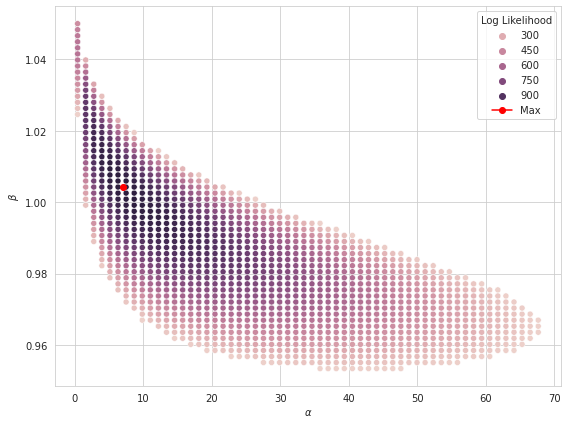
\includegraphics[width=0.75\textwidth]{hw5-1.png}
  \captionsetup{justification=centering}
  \caption{}
\end{figure*}

\paragraph{(c)}
\paragraph{(d)}

\section{Chapter 3 Ex 2}
\paragraph{(a)}
\paragraph{(b)}
\paragraph{(c)}
\paragraph{(d)}
\paragraph{(e)}

\section{Chapter 3 Ex 3}
\paragraph{(a)}
\paragraph{(b)}
\paragraph{(c)}

\end{document}